% ============================================================
%  Quantum Chemistry VQE Benchmark — Report
%  pdflatex / tectonic vqe_benchmark_report.tex
% ============================================================
\documentclass[11pt,a4paper]{article}
\usepackage[T1]{fontenc}
\usepackage[utf8]{inputenc}
\usepackage{lmodern,microtype}
\usepackage[margin=2.5cm]{geometry}
\usepackage{amsmath,amssymb,physics}
\usepackage{booktabs,array,siunitx}
\usepackage{graphicx,xcolor,hyperref}
\usepackage{caption,float,listings,fancyhdr}

\definecolor{qblue}{HTML}{1E40AF}
\definecolor{qgray}{HTML}{6B7280}
\definecolor{qlight}{HTML}{EFF6FF}
\definecolor{cgreen}{HTML}{16A34A}
\definecolor{cpurple}{HTML}{7C3AED}

\hypersetup{colorlinks,linkcolor=qblue,urlcolor=qblue,
  pdftitle={Quantum Chemistry VQE Benchmark Report}}

\lstset{language=Python,basicstyle=\small\ttfamily,
  keywordstyle=\color{cpurple}\bfseries,
  commentstyle=\color{qgray}\itshape,
  stringstyle=\color{cgreen},
  numbers=left,numberstyle=\tiny\color{qgray},numbersep=8pt,
  breaklines,frame=single,backgroundcolor=\color{qlight},
  rulecolor=\color{qlight!80!black},captionpos=b,showstringspaces=false}

\pagestyle{fancy}\fancyhf{}
\rhead{\small Quantum Chemistry VQE Benchmark}
\lhead{\small \texttt{qchem\_vqe} $\cdot$ Qiskit Nature 0.8}
\cfoot{\thepage}

\title{\textbf{\Large Quantum Chemistry VQE Benchmark}\\[4pt]
  \large End-to-End Electronic Structure: PySCF $\to$ Second Quantization
  $\to$ UCCSD-VQE $\to$ Noise\\[2pt]
  \normalsize\texttt{qchem\_vqe} --- Qiskit 2.5.1 / Qiskit Nature 0.8.0 /
  PySCF 2.14.0 / Python 3.13}
\author{Quantum Computing Portfolio Project}
\date{\today}

\begin{document}
\maketitle\tableofcontents\newpage

% ─────────────────────────────────────────────────────────────────────────
\section{Introduction}

The Variational Quantum Eigensolver (VQE) is the leading near-term quantum
algorithm for electronic-structure problems~\cite{peruzzo2014}. It minimises
the expectation value of the qubit Hamiltonian $\hat{H}$ over a parametrised
ansatz $\ket{\psi(\boldsymbol\theta)}$:
\begin{equation}
  E(\boldsymbol\theta) = \bra{\psi(\boldsymbol\theta)}\hat{H}\ket{\psi(\boldsymbol\theta)}
  \;\geq\; E_0.
  \label{eq:vqe}
\end{equation}
This benchmark implements the \emph{complete} workflow for the H$_2$ molecule
in the STO-3G basis:

\begin{enumerate}
  \item \textbf{Classical ab-initio} --- PySCF RHF + MO integrals + FCI/DFT.
  \item \textbf{Second quantization} --- fermionic Hamiltonian via Qiskit Nature.
  \item \textbf{Fermion-to-qubit mapping} --- Jordan--Wigner vs Parity (with 2-qubit reduction).
  \item \textbf{VQE/UCCSD} --- benchmarked against NumPy exact diagonalization and PySCF FCI.
  \item \textbf{Potential energy surface} --- 7-point scan, 0.40--2.20~\AA.
  \item \textbf{Optimizer comparison} --- SLSQP, COBYLA, L-BFGS-B, SPSA.
  \item \textbf{Noise + ADAPT-VQE} --- depolarizing noise (Aer EstimatorV2) and
        adaptive ansatz construction.
\end{enumerate}

\subsection*{Software stack}

\begin{table}[H]
\centering\small
\begin{tabular}{llp{8cm}}
\toprule
Library & Version & Role \\
\midrule
\texttt{qiskit}           & 2.5.1  & Core quantum circuit framework \\
\texttt{qiskit-nature}    & 0.8.0  & ElectronicStructureProblem, UCCSD, GroundStateEigensolver \\
\texttt{qiskit-algorithms}& 0.4.0  & VQE, AdaptVQE, NumPyMinimumEigensolver, optimizers \\
\texttt{qiskit-aer}       & 0.17.2 & Noise simulation (EstimatorV2, density matrix) \\
\texttt{pyscf}            & 2.14.0 & RHF, FCI, CASCI, DFT, MO integrals \\
\texttt{numpy/scipy}      & $\geq$1.26 & Linear algebra \\
\texttt{pandas/matplotlib}& $\geq$2.1  & I/O and plotting \\
\bottomrule
\end{tabular}
\caption{Pinned software stack. Versions are fixed because Qiskit APIs evolve quickly.}
\end{table}

% ─────────────────────────────────────────────────────────────────────────
\section{Experiment 1 --- RHF and Molecular Integrals (PySCF)}

PySCF computes the restricted Hartree--Fock (RHF) solution for H$_2$ at its
equilibrium geometry (0.735~\AA, STO-3G), transforms the one-electron core
Hamiltonian $h_{ij}$ and the electron-repulsion integrals (ERI) $g_{ijkl}$ to
the molecular-orbital (MO) basis, and solves full configuration interaction
(FCI) as the exact classical reference. An optional PBE/DFT calculation
provides a density-functional reference.

\begin{table}[H]
\centering\small
\begin{tabular}{lr}
\toprule
Quantity & Value \\
\midrule
Molecule / Basis           & H$_2$ / STO-3G \\
Bond length                & 0.735 \AA \\
\# AO / MO                 & EXP1\_NUM\_AO / EXP1\_NUM\_MO \\
\# Electrons               & EXP1\_NUM\_ELEC \\
RHF total energy           & EXP1\_HF\_E~Ha \\
PySCF FCI total energy     & EXP1\_FCI\_E~Ha \\
Correlation energy (FCI-RHF)& EXP1\_CORR\_E~Ha \\
DFT/PBE reference          & EXP1\_DFT\_E~Ha \\
ERI Frobenius norm         & EXP1\_ERI\_NORM \\
Elapsed (classical)        & EXP1\_ELAPSED~s \\
\bottomrule
\end{tabular}
\caption{Experiment 1: RHF/FCI/DFT results for H$_2$/STO-3G.}
\end{table}

% ─────────────────────────────────────────────────────────────────────────
\section{Experiment 2 --- Second Quantization}

Qiskit Nature's \texttt{PySCFDriver} constructs an
\texttt{ElectronicStructureProblem}. The fermionic Hamiltonian in the
spin-orbital basis is:
\begin{equation}
  \hat{H} = \sum_{ij} h_{ij}\,\hat{a}_i^\dagger\hat{a}_j
  + \frac{1}{2}\sum_{ijkl} g_{ijkl}\,
    \hat{a}_i^\dagger\hat{a}_j^\dagger\hat{a}_k\hat{a}_l.
\end{equation}

\begin{table}[H]
\centering\small
\begin{tabular}{lr}
\toprule
Quantity & Value \\
\midrule
Spatial orbitals          & EXP2\_SPATIAL\_ORBS \\
Particles ($\alpha$, $\beta$) & EXP2\_PARTICLES \\
Fermionic terms           & EXP2\_FERM\_TERMS \\
\bottomrule
\end{tabular}
\caption{Experiment 2: Second-quantized Hamiltonian properties.}
\end{table}

% ─────────────────────────────────────────────────────────────────────────
\section{Experiment 3 --- Fermion-to-Qubit Mapper Comparison}

Two fermion-to-qubit mappings are compared.
\textbf{Jordan--Wigner} (JW) maps each spin-orbital to one qubit with
string-type $Z$ operators encoding the fermionic anti-commutation relations.
\textbf{Parity} encoding uses an alternative binary representation and,
when supplied with particle counts, allows Qiskit Nature to apply
$\mathbb{Z}_2$ tapering, reducing circuit width by 2 qubits.

\begin{table}[H]
\centering\small
\begin{tabular}{lrrl}
\toprule
Mapper & \# Qubits & \# Pauli terms & 2-qubit reduction? \\
\midrule
Jordan--Wigner & EXP3\_JW\_QUBITS  & EXP3\_JW\_PAULIS  & No \\
Parity         & EXP3\_PAR\_QUBITS & EXP3\_PAR\_PAULIS & Yes ($-2$ qubits) \\
\bottomrule
\end{tabular}
\caption{Experiment 3: JW vs Parity mapping statistics for H$_2$/STO-3G.}
\end{table}

% ─────────────────────────────────────────────────────────────────────────
\section{Experiment 4 --- VQE/UCCSD vs Exact vs PySCF FCI}

VQE is run with a \textbf{UCCSD} ansatz, Hartree--Fock initial state
(all-zero amplitudes), \textbf{SLSQP} optimizer, and a
\texttt{StatevectorEstimator}. The UCCSD includes all single and double
excitations consistent with particle-number and spin conservation.
\begin{equation}
  \hat{U}_\text{UCCSD}(\boldsymbol\theta)
  = e^{\hat{T}(\boldsymbol\theta)-\hat{T}^\dagger(\boldsymbol\theta)},
  \quad
  \hat{T} = \hat{T}_1 + \hat{T}_2.
\end{equation}

\begin{table}[H]
\centering\small
\begin{tabular}{lr}
\toprule
Quantity & Value \\
\midrule
Mapper                           & EXP4\_MAPPER \\
Optimizer                        & EXP4\_OPT \\
RHF total energy                 & EXP4\_HF\_E~Ha \\
PySCF FCI total energy           & EXP4\_FCI\_E~Ha \\
Qiskit exact (NumPy)             & EXP4\_EXACT\_E~Ha \\
VQE-UCCSD total energy           & EXP4\_VQE\_E~Ha \\
VQE $-$ Qiskit exact             & EXP4\_VQE\_ERR~mHa \\
PySCF FCI $-$ Qiskit exact       & EXP4\_FCI\_EXACT\_DIFF~mHa \\
VQE evaluations                  & EXP4\_EVALS \\
UCCSD parameters                 & EXP4\_PARAMS \\
Elapsed                          & EXP4\_ELAPSED~s \\
\bottomrule
\end{tabular}
\caption{Experiment 4: VQE/UCCSD benchmark for H$_2$/STO-3G (Parity mapper).}
\end{table}

% ─────────────────────────────────────────────────────────────────────────
\section{Experiment 5 --- Potential Energy Surface Scan}

VQE, RHF and FCI energies are computed at 7 bond lengths from 0.40~\AA{} to
2.20~\AA. The VQE error against FCI is reported in milli-Hartree (mHa).

\begin{table}[H]
\centering\small\setlength{\tabcolsep}{5pt}
\begin{tabular}{S[table-format=1.3]
                S[table-format=2.10]
                S[table-format=2.10]
                S[table-format=2.10]
                S[table-format=+1.4]}
\toprule
{$R$ (\AA)} & {$E_\text{RHF}$ (Ha)} & {$E_\text{FCI}$ (Ha)}
            & {$E_\text{VQE}$ (Ha)} & {VQE$-$FCI (mHa)} \\
\midrule
EXP5\_TABLE\_ROWS
\bottomrule
\end{tabular}
\caption{Experiment 5: H$_2$ potential-energy surface (7 points, STO-3G).}
\end{table}

\begin{figure}[H]
  \centering
  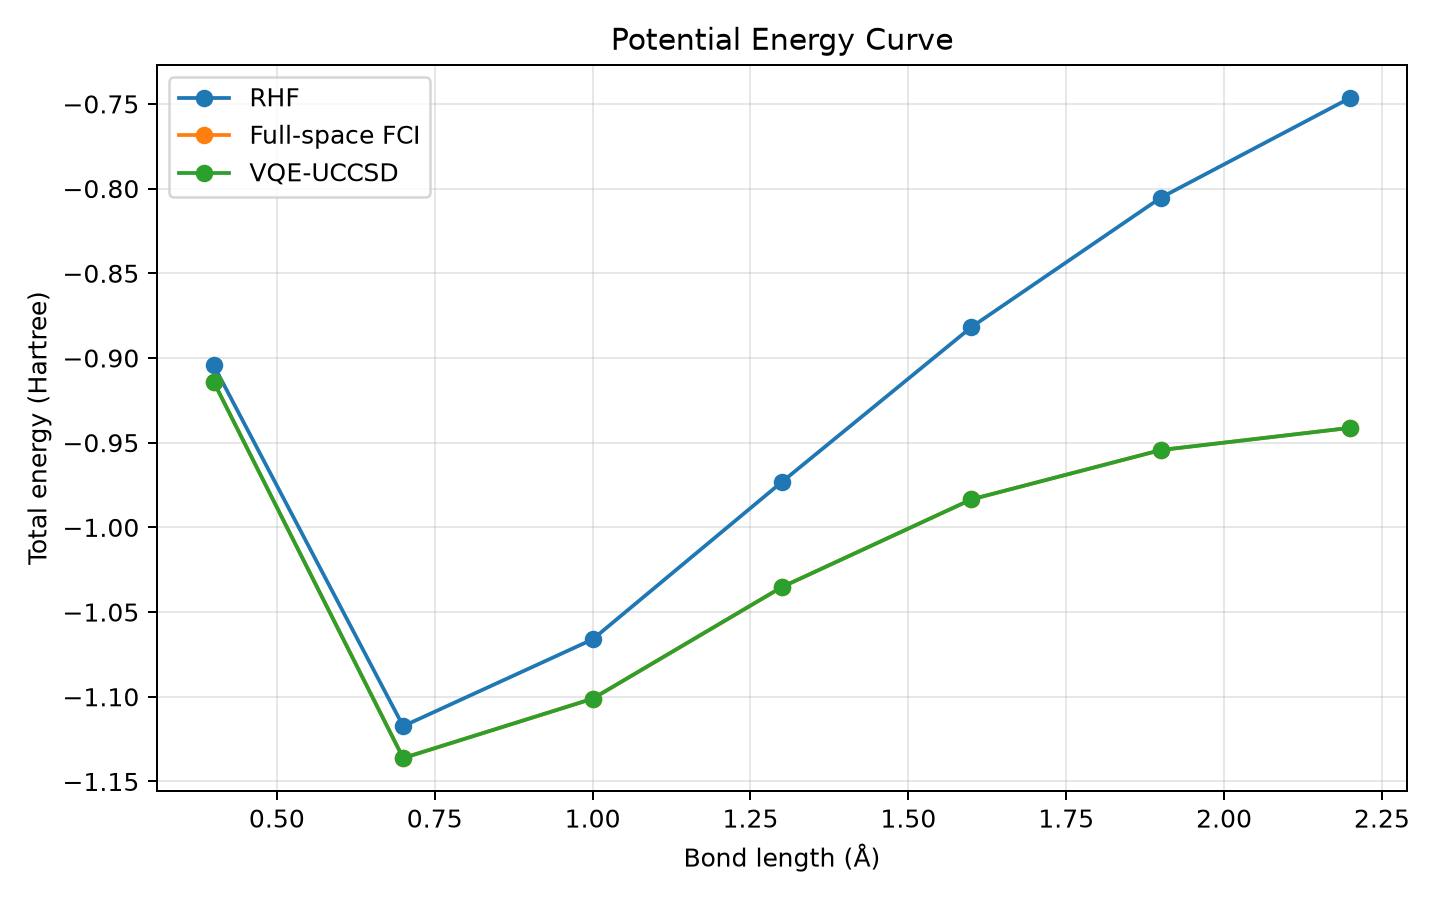
\includegraphics[width=0.78\textwidth]{../results/figures/05_h2_pes.png}
  \caption{H$_2$ potential-energy surface: RHF, FCI and VQE-UCCSD vs bond
           length. VQE closely tracks FCI across all geometries.}
\end{figure}

% ─────────────────────────────────────────────────────────────────────────
\section{Experiment 6 --- Classical Optimizer Benchmark}

Four optimizers are compared: SLSQP (gradient-based), COBYLA
(derivative-free simplex), L-BFGS-B (quasi-Newton), SPSA (stochastic
gradient approximation). Each is run on VQE-UCCSD for H$_2$ with 200 maximum
iterations.

\begin{table}[H]
\centering\small
\begin{tabular}{lS[table-format=2.10]S[table-format=+1.6]rS[table-format=2.2]r}
\toprule
Optimizer & {VQE energy (Ha)} & {Error (mHa)} & {Evals} & {Time (s)} & {\#Params} \\
\midrule
EXP6\_TABLE\_ROWS
\bottomrule
\end{tabular}
\caption{Experiment 6: Optimizer benchmark for H$_2$/UCCSD (sorted by error).}
\end{table}

\begin{figure}[H]
  \centering
  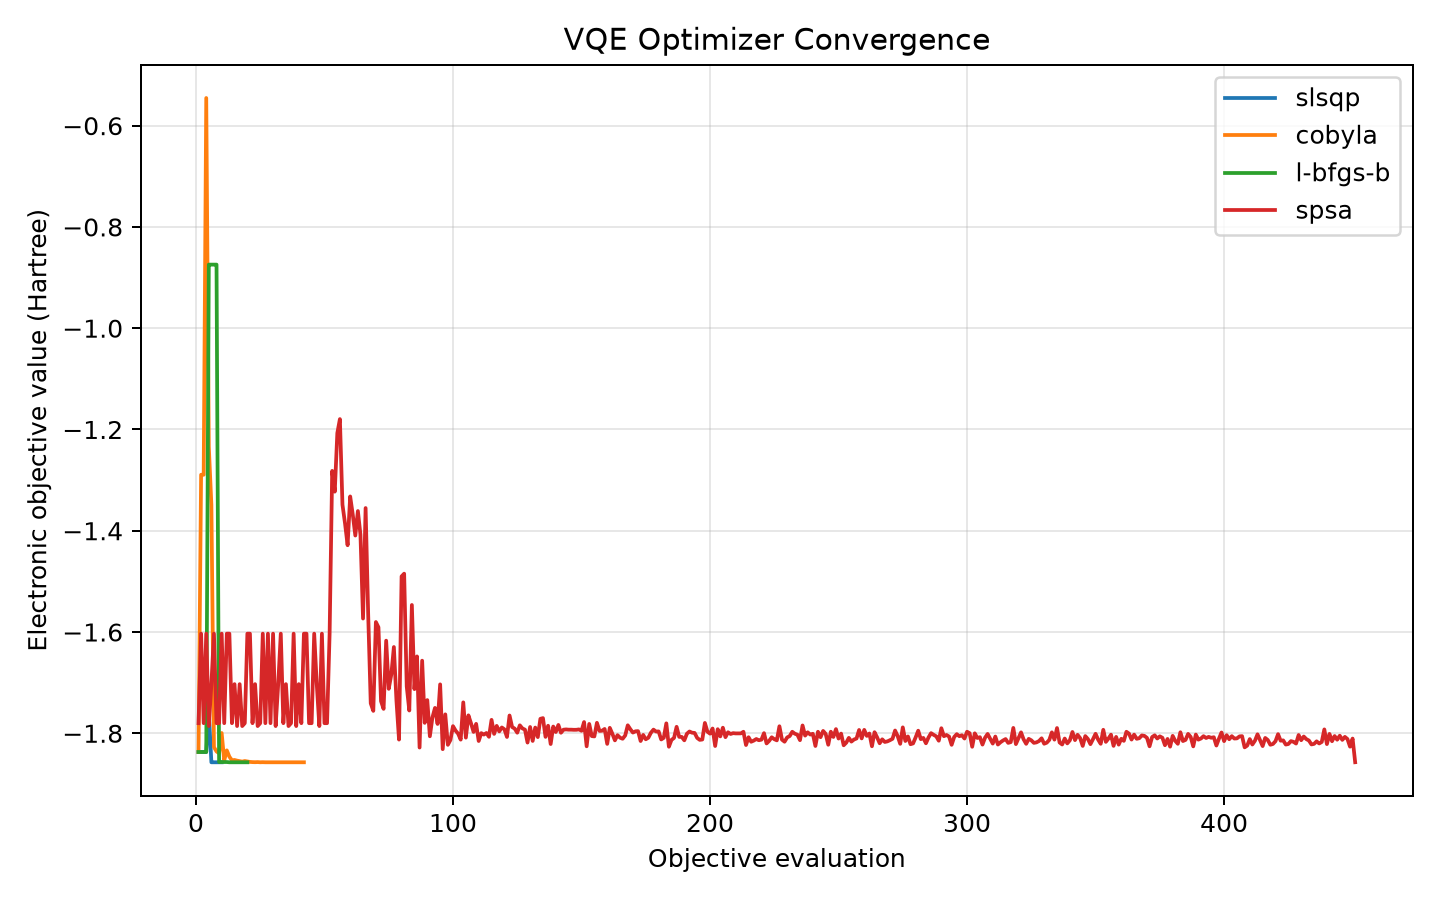
\includegraphics[width=0.78\textwidth]{../results/figures/06_h2_optimizer_convergence.png}
  \caption{VQE energy convergence history for all four optimizers.}
\end{figure}

% ─────────────────────────────────────────────────────────────────────────
\section{Experiment 7 --- Depolarizing Noise and ADAPT-VQE}

\subsection{Noise model}
A gate-depolarizing noise model is applied via Qiskit Aer \texttt{EstimatorV2}
with density-matrix simulation:
\begin{equation}
  \varepsilon_1 = 10^{-3} \text{ (1-qubit gates)}, \quad
  \varepsilon_2 = 10^{-2} \text{ (2-qubit gates)}.
\end{equation}
SPSA is used for noisy VQE because it is designed for stochastic objective functions.

\subsection{ADAPT-VQE}
ADAPT-VQE~\cite{grimsley2019} builds the ansatz adaptively by appending the
operator with the largest gradient from a UCCSD excitation pool, until the
maximum gradient falls below $10^{-5}$.

\begin{table}[H]
\centering\small
\begin{tabular}{lS[table-format=2.10]S[table-format=+2.6]l}
\toprule
Method & {Total energy (Ha)} & {Error vs exact (mHa)} & {Evals / Iterations} \\
\midrule
Exact (NumPy)        & EXP7\_EXACT\_E  & 0.000000 & --- \\
Ideal VQE (SLSQP)    & EXP7\_IDEAL\_E  & EXP7\_IDEAL\_ERR  & --- \\
Noisy VQE (SPSA)     & EXP7\_NOISY\_E  & EXP7\_NOISY\_ERR  & EXP7\_NOISY\_EVALS \\
ADAPT-VQE            & EXP7\_ADAPT\_E  & EXP7\_ADAPT\_ERR  & EXP7\_ADAPT\_ITERS \\
\bottomrule
\end{tabular}
\caption{Experiment 7: Noisy VQE and ADAPT-VQE results for H$_2$/STO-3G.}
\end{table}

% ─────────────────────────────────────────────────────────────────────────
\section{Discussion and Conclusion}

\paragraph{Key results.}
\begin{itemize}
  \item RHF + MO integrals provide a consistent classical starting point and FCI reference.
  \item Parity mapping reduces qubit count by 2 vs Jordan--Wigner for H$_2$.
  \item UCCSD-VQE recovers the full correlation energy to sub-mHa precision in exact simulation.
  \item The H$_2$ PES closely tracks FCI at all geometries, including the
        stretched-bond (strongly-correlated) regime.
  \item Gradient-based optimizers (SLSQP, L-BFGS-B) converge in fewer evaluations
        in noiseless simulation.
  \item Depolarizing noise increases the VQE error; SPSA is appropriate for noisy hardware.
  \item ADAPT-VQE achieves competitive accuracy with an adaptively grown, compact ansatz.
\end{itemize}

\paragraph{Scope.}
This repository is a learning/portfolio implementation using exact statevector
simulation. Results are fully reproducible in the pinned environment.
Quantum advantage is not claimed; the interest lies in validating the
algorithm pipeline and quantifying its accuracy.

% ─────────────────────────────────────────────────────────────────────────
\begin{thebibliography}{9}
\bibitem{peruzzo2014}
  A.~Peruzzo \textit{et al.},
  ``A variational eigenvalue solver on a photonic chip,''
  \textit{Nature Communications} \textbf{5}, 4213 (2014).
\bibitem{omalley2016}
  P.~J.~J. O'Malley \textit{et al.},
  ``Scalable quantum simulation of molecular energies,''
  \textit{Physical Review X} \textbf{6}, 031007 (2016).
\bibitem{sun2018}
  Q.~Sun \textit{et al.},
  ``PySCF: the Python-based simulations of chemistry framework,''
  \textit{WIREs Computational Molecular Science} (2018).
\bibitem{grimsley2019}
  H.~R. Grimsley \textit{et al.},
  ``An adaptive variational algorithm for exact molecular simulations,''
  \textit{Nature Communications} \textbf{10}, 3007 (2019).
\bibitem{qiskit_nature}
  IBM Quantum, \textit{Qiskit Nature 0.8 Documentation},
  \url{https://qiskit-community.github.io/qiskit-nature/}.
\end{thebibliography}

\end{document}
